\section{Our Techniques}\label{sec:our-techniques}

We now explain the main differences between the polynomial computations carried on during the rounds of the vanilla STARK (Section \ref{sec:vanilla-STARK}) and our protocol. We also explain the tradeoffs arising from controlling the constraint degree either at the representation of the AIR or inside the protocol itself.


%%%%%%%%%%%%%%%%%%%%%%%%%%%%%%%%%%%%%%%%%%%%%%%%%%%%%%%%%%%%%%%
\subsection{Commiting to Multiple Polynomial at Once}\label{sec:committing}

In our protocol, the prover sends Merkle tree commitments to multiple polynomials in each round. The naive way of proceeding is by sending one Merkle tree root per polynomial. In this section, we explain how we achieve a sound alternative by computing a single Merkle tree of all polynomials in each round. Our strategy not only reduces the amount of Merkle roots that \P has to send to \V in each round but also reduces the Merkle paths that \P needs to send to \V when \P gets asked for evaluations of multiple polynomials at the same point.

\paragraph*{Notation.} As explained in Section \ref{sec:vanilla-STARK}, commitments are generated by computing Merkle trees over polynomial evaluations over a nontrivial coset $H$ of a cyclic subgroup of $\FF^*$ with order $m$. For this section, explicitly set $H = \{h_1,h_2,h_3,\dots,h_m\}$.

Say that $f_1,\dots,f_N \in \KK_{<n}[X]$ is the set of polynomials that we want to construct the Merkle Tree on. More precisely, we want to compute the Merkle tree over the following $m \times N$ matrix of polynomial evaluations:
\[
\left(
\begin{array}{cccc}
f_1(h_1), & f_2(h_1), &\dots, &f_N(h_1) \\[0.1cm]
f_1(h_2), & f_2(h_2), &\dots, &f_N(h_2) \\
\vdots &\vdots &\cdots & \vdots \\
f_1(h_m), & f_2(h_m), & \dots, &f_N(h_m) \\
\end{array}
\right)
\]

We start the construction of the Merkle Tree by grouping the evaluations of $f_1,\dots,f_N$ at a single point of $H$. That is, the $i$-th leaf of the Merkle tree is formed by (the hash of) the $i$-th row of the previous matrix. This gives a total of $m$ leaves, which is by assumption a power of two. To be more precise, the leaf elements of the Merkle Tree, indexed by the corresponding $H$-value, will consist on:
\[
\begin{array}{|ccc|}
\hline
\text{leaf } h_1 & \Longrightarrow & \H(f_1(h_1), f_2(h_1), \dots, f_N(h_1)) \\[0.1cm]
\text{leaf } h_2 & \Longrightarrow & \H(f_1(h_2), f_2(h_2), \dots, f_N(h_2)) \\
\vdots &  & \vdots \\[0.1cm]
\text{leaf } h_m & \Longrightarrow & \H(f_1(h_m), f_2(h_m), \dots, f_N(h_m)) \\
\hline
\end{array}
\]
where $\H$ is any collision-resistant hash function. Once all the leaves are computed, the rest of the Merkle tree is computed, as usual, by recursively hashing the concatenation of its two child nodes until the Merkle root is achieved. The commitments to $f_1,\dots,f_N$ is this single Merkle root. 

Now, notice how if \V requests a Merkle proof for the evaluation of all $f_1,\dots,f_N$ at a single point $h_i$, \P can prove the consistency of all the evaluations $f_1(h_i),\dots,f_N(h_i)$ with the Merkle root by simply sending the Merkle path corresponding to the leaf containing such evaluations. Compared to the naive version, this version improves the proof size from $O(N\log m)$ elements down to $O(\log m)$ elements. This will be convenient for the batched FRI execution of our protocol, where we group evaluations of a set of polynomials at a single point for succinctly answering each batched consistency check. 


\ifPOLYGON
To be more specific, the hash function $H$ is set to be the Poseidon \cite{USENIX:GKRRS21} hash function. Poseidon was chosen because it was created to minimize prover and verifier complexities when zero-knowledge proofs are generated and validated. Notably, the best hashing performance is obtained when the state size is limited to $12$ field elements, $4$ of which are occupied by the capacity of the hash function. This implies that to get the best Poseidon performance, we have to restrict the input size to be of $8$ field elements.

Leaf hashes are computed ``linearly''. By linearly we mean that, if the input to the hash function is $t_1(sh^i)$, $t_2(sh^i)$, $\dots$, $t_N(sh^i)$, then we process it as follows:
\begin{enumerate}
	\item The input is split in chunks of $8$ elements, filling with repetitions of the $0$ element if $N$ is not a multiple of $8$.
	\item The first chunk is hashed using Poseidon with capacity $(0, 0, 0, 0)$.
	\item The following chunk is hashed using Poseidon with the capacity being the output of the previous hash.
	\item Go to Step 3 until there are no more chunks.
\end{enumerate}

An example of this process can be seen in Figure \ref{fig:linear-hash}.
\begin{figure}[h!]
	\centering
	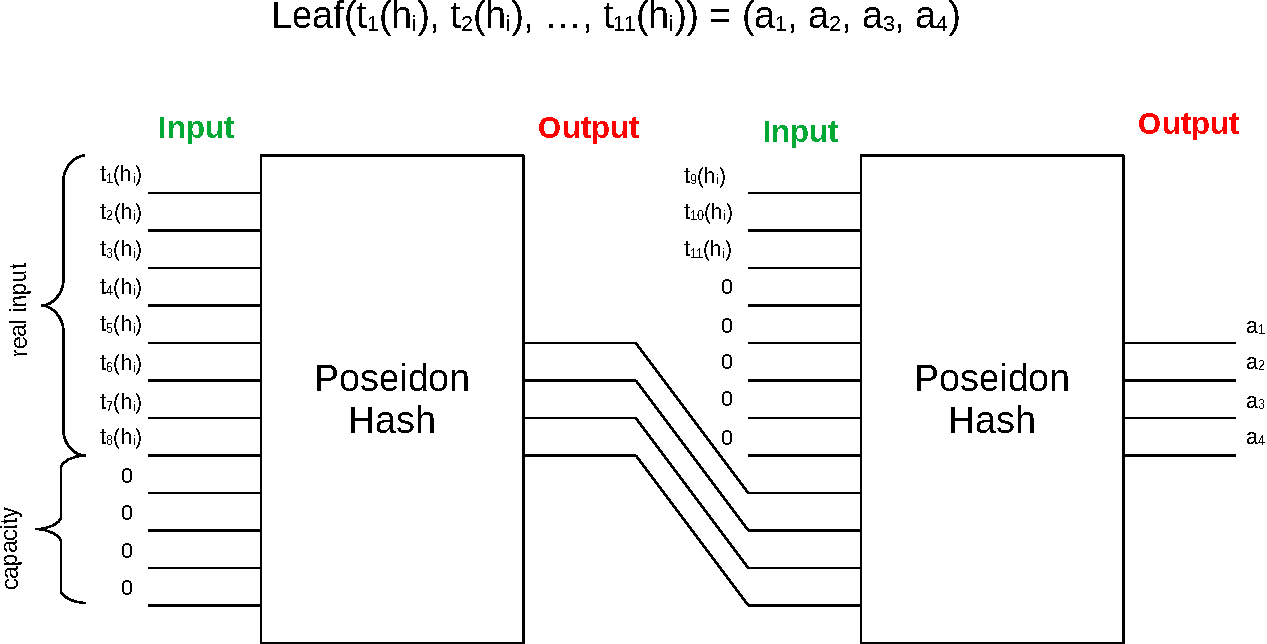
\includegraphics[width=.7\textwidth]{../figures/poseidon-linear-hash}
	\caption{Leaf hash computation on input $(t_1(sh^i), \dots, t_{11}(sh^i))$ in a linear manner.}
	\label{fig:linear-hash}
\end{figure}

Once all the hashed leaves are obtained, one starts to construct the Merkle tree by continually hashing two child nodes using Poseidon with capacity $(0,0,0,0)$ and defining the parent node as the output. This is well defined because Poseidon's output consists of $4$ field elements, while its input size consists of $8$. See Figure \ref{fig:full-poseidon} for an example with $4$ leaves.
\begin{figure}[H]
	\centering
	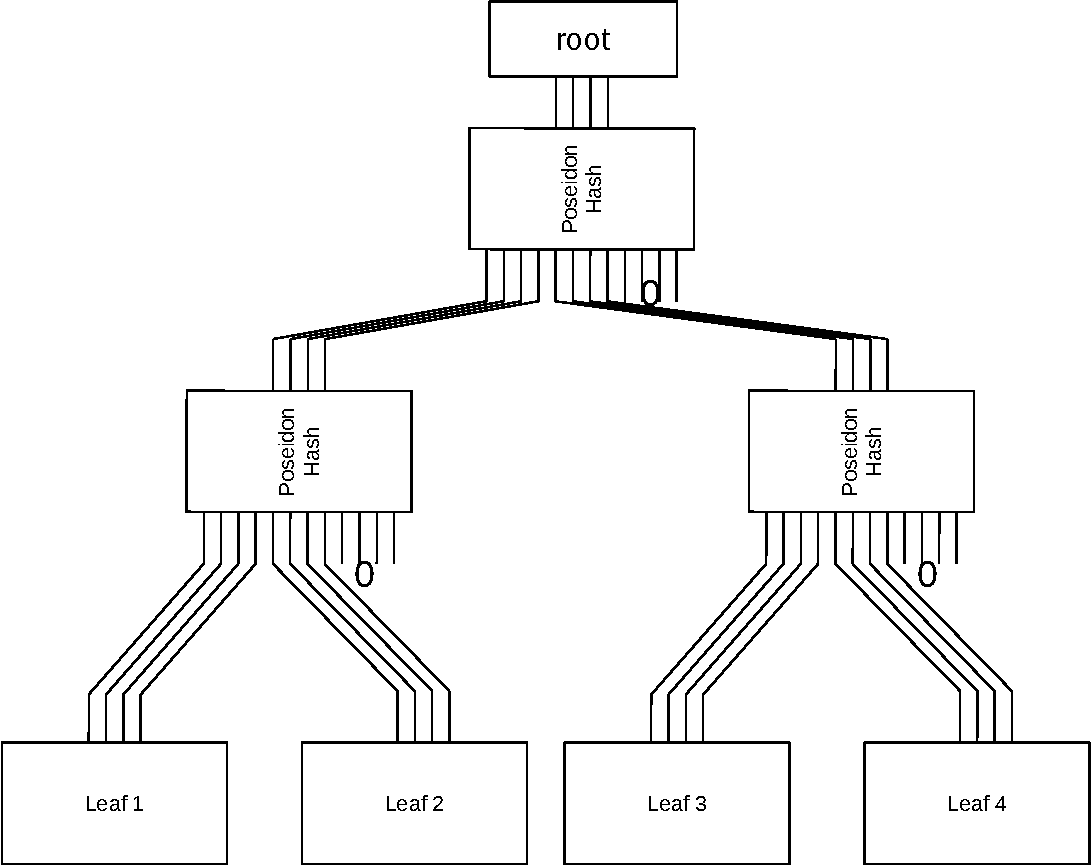
\includegraphics[width=.6\textwidth]{../figures/MT-poseidon-example}
	\caption{Merkle's tree hash computation assuming $4$ leafs.}
	\label{fig:full-poseidon}
\end{figure}

This procedure has been extended to being able to compute hashes faster using several GPUs. First of all, we are splitting all our polynomials in $4$ chunks of size:
\[
\mathtt{batchSize} = \Biggl\lfloor \max \left( 8, \frac{N + 3}{4} \right)  \Biggr\rfloor.
\]

Of course, it may be possible that not all of the chunks have exactly this amount of elements. In this case, we prioritize filling the first $3$ ones up to this size, letting the last one become smaller, but not so smaller. The idea is that, with the formula above, the chunk size is increased by $1$ once $N$ increases by $4$ (when $N > 32$, which is the first time when all chunks have exactly \texttt{batchSize} number of elements). Hence, for $N$ big enough, the last chunk never will become smaller than $\mathtt{batchSize} - 3$, becoming an almost uniform distribution of the polynomials among the $4$ chunks. Table \ref{tab:multi-gpu-chunks} shows several examples of how these chunk division sizes look like.

\begin{figure}[h!]
	\centering
	\[
	\begin{array}{|c|c|c|c|c|c|}
	\hline
	N	&\texttt{batchSize}	&\textbf{Chunk 1}	&\textbf{Chunk 2}	&\textbf{Chunk 3}	&\textbf{Chunk 4}	\\
	\hline
	1		&8			&1				&0				&0				&0				\\
	\cdots	&\cdots		&\cdots			&\cdots			&\cdots			&\cdots			\\
	8		&8			&8				&0				&0				&0				\\
	9		&8			&8				&1				&0				&0				\\
	10		&8			&8				&2				&0				&0				\\
	\cdots	&\cdots     &\cdots			&\cdots			&\cdots			&\cdots			\\
	17		&8			&8				&8				&1				&0				\\
	\cdots	&\cdots		&\cdots			&\cdots			&\cdots			&\cdots			\\
	25		&8			&8				&8				&8				&1				\\
	\cdots	&\cdots		&\cdots			&\cdots			&\cdots			&\cdots			\\
	32		&8			&8				&8				&8				&8				\\
	33		&9			&9				&9				&9				&6				\\
	34		&9			&9				&9				&9				&7				\\
	35		&9			&9				&9				&9				&8				\\
	36		&9			&9				&9				&9				&9				\\
	37		&10			&10				&10				&10				&7				\\
	38		&10			&10				&10				&10				&8				\\
	\cdots	&\cdots		&\cdots			&\cdots			&\cdots			&\cdots			\\
	51		&13			&13				&13				&13				&12				\\
	\cdots	&\cdots		&\cdots			&\cdots			&\cdots			&\cdots			\\
	\hline
	\end{array}
	\]
	\caption{Chunk's size distribution for several values of $N$.}
	\label{tab:multi-gpu-chunks}
\end{figure}

After the polynomial splitting in $4$ chunks (say $T_1, T_2, T_3$ and $T_4$), we perform the previously defined linear hash of all of them in a parallel way, ending up with a set of a maximum amount of $16$ field elements corresponding to the $4$ outputs of $4$ field elements each. To finish this updated version of the linear hash, we perform the linear hash of these $16$ elements as done previously, which outputs a final total amount of $4$ field elements. More precisely, if 
\[
LH(T_i) = (H_{i, 1}, H_{i, 2}, H_{i, 3}, H_{i, 4})	\quad i \in \{1, 2, 3, 4\},
\]
then the final output will be
\[
\scalebox{0.85}{\mbox{\ensuremath{\displaystyle 
			LH(H_{1, 1}, H_{1, 2}, H_{1, 3}, H_{1, 4}, H_{2, 1}, H_{2, 2}, H_{2, 3}, H_{2, 4}, H_{3, 1}, H_{3, 2}, H_{3, 3}, H_{3, 4}, H_{4, 1}, H_{4, 2}, H_{4, 3}, H_{4, 4})
}}},
\]
where $LH$ denotes the single-GPU version of the linear hash. 



\subsection{Transcript Generation and Computing Verifier Challenges}\label{sec:transcript-gen}

We will describe our protocol version as a non-interactive protocol using the Fiat-Shamir heuristic \cite{C:FiaSha86}. Therefore, we need to specify how we are generating the random challenges from $\KK$ (or equivalently, $3$ elements of $\FF$). Through all this section we will use an instance of a Poseidon hash function having state size of $12$ field elements ($8$ for inputs and $4$ for capacity) and output size of $12$ field elements. 

The strategy for generating the transcript is similar to the linear hash strategy described before. Suppose we want to add $c_1, \dots, c_r$ elements to the transcript. We proceed as follows:

\begin{enumerate}

\item The input is split in chinks of $8$ field elements, filling with repetitions of the $0$ element if $r$ is not a multiple of $8$. 

\item The first chunk is hashed using Poseidon with capacity $(0,0,0,0)$.

\item The following chunk is hashed using Poseidon with the capacity being the $4$ last elements of the output of the previous hash. 

\item Go to Step $3$ until there are no more chunks. 

\end{enumerate}

Observe that the $8$ remaining elements of each hash output are not being used until we stop the loop between the steps $3$ and $4$. We depict the previous strategy in Figure \ref{fig:transcript-gen}.  

\begin{figure}[h!]
\centering
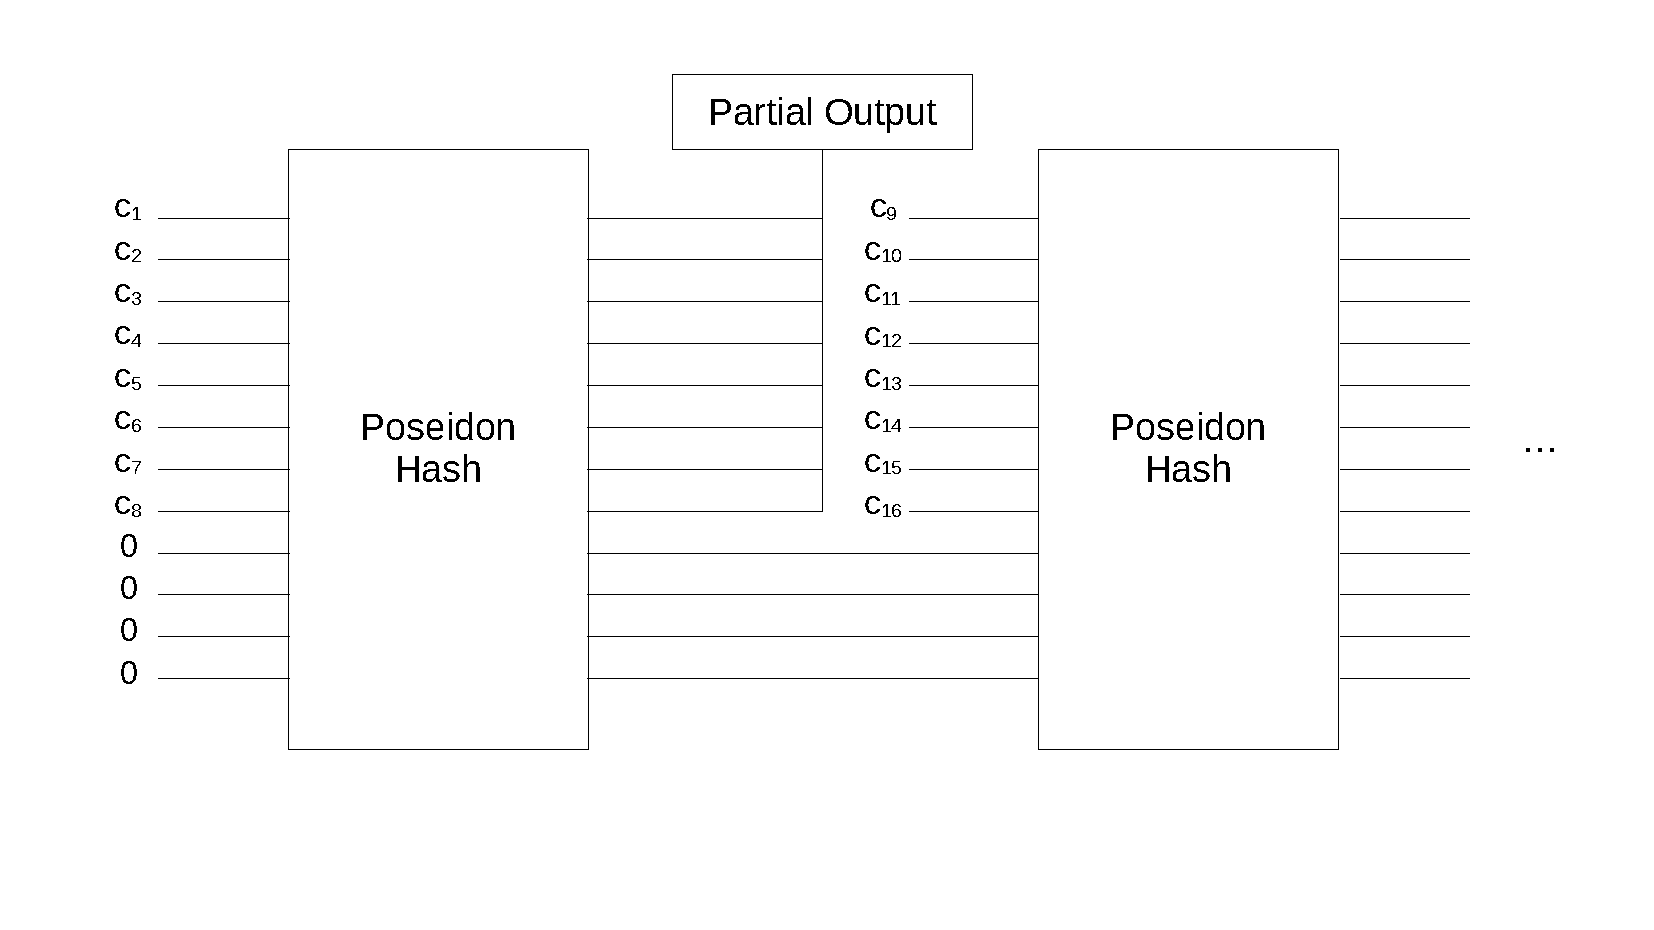
\includegraphics[width=.8\textwidth]{../figures/transcript}
\caption{First two steps of the transcript generation.}
\label{fig:transcript-gen}
\end{figure}

When we stop adding elements to the transcript, we end up with an output consisting in $8$ field elements, say $(t_1, \dots, t_8)$. For a given transcript state we can extract at most $3$ challenges of $\KK$. The first two elements are trivially obtained
\[
t_1 + t_2 \varphi + t_3 \varphi^2, \quad t_4 + t_5 \varphi + t_6 \varphi^2
\]
for $\varphi$ being a root of the irreducible polynomial used to construct $\KK$ from $\FF$. Since we do not have enough elements to construct a third extension field element, we proceed as follows. We construct an field element $t_9$ hashing $8$ zeros with the capacity being the last $4$ output elements of the last hash performed at the time of generating the transcript (that is, the elements that will become the capacity of the next hash when adding a new element into the transcript). Hence, we get a third element in $\KK$
\[
t_7 + t_8 \varphi + t_9 \varphi^2.
\]
However, observe that we can not extract more than that. 

We will denote by \transcript the transcript instance and we will define for it the following operations:

\begin{itemize}

\item \textbf{Add:} Having elements $c_1, \dots, c_r \in \FF$, we denote by 
\[
\transcriptAdd(c_1, \dots, c_r)
\]
the operation of adding $c_1, \dots, c_r$ to the transcript using the previous procedure. 

\item \textbf{Extract:} Having a transcript state \textsf{T}, we denote by
\[
\transcriptExtract{i}(\transcript) \in \KK \quad i \in \{1, 2, 3\}
\]
the result of extracting a single extension field $\KK$ element from it using the previously described procedure. Using the notation above:
\begin{align*}
&\transcriptExtract{1}(\transcript) = t_1 + t_2 \varphi + t_3 \varphi^2, \\
&\transcriptExtract{2}(\transcript) = t_4 + t_5 \varphi + t_6 \varphi^2, \\
&\transcriptExtract{3}(\transcript) = t_7 + t_8 \varphi + t_9 \varphi^2.
\end{align*}
\end{itemize}

A proof that the resulting non-interactive protocol is knowledge sound after applying the Fiat-Shamir using this strategy can be found, for example, in Theorem 4 of \cite{EPRINT:AttFehKlo21}.

\fi



%%%%%%%%%%%%%%%%%%%%%%%%%%%%%%%%%%%%%%%%%%%%%%%%%%%%%%%%%%%%%%%
\subsection{Preprocessed Polynomials and Public Values}\label{sec:preprocessed-public}

Among the set of polynomials that are part of the polynomial constraint system representing the problem's statement, we differentiate between two types: \textit{committed polynomials} and \textit{preprocessed polynomials}. 

Committed polynomials are those polynomials for which the verifier only has oracle access and are therefore committed (via Merkle trees) by the prover before the verifier starts querying them. In other words, these polynomials can only be known, in principle, in their entire form by the prover of the protocol. Consequently, the verifier is limited to knowing a ``small fraction'' of these polynomials' evaluations. In practice, this fraction is randomly chosen by the verifier and is proportional to the number of oracle queries that the verifier makes to the particular polynomial. For the shake of the protocols to be scalable, the number of queries made to committed polynomials should be at most logarithmic in their degree. An example of committed polynomials is trace columns polynomials $\tr_i$.

On the other hand, preprocessed polynomials are known by the verifier in their entirety even before the execution of the protocol. More precisely, once a polynomial constraint system $\C$ is fixed, the verifier has complete access (either in coefficient form or in evaluation form) to the set of preprocessed polynomials. As with committed polynomials, the verifier ends up needing only a small subset of evaluations of such polynomials during the protocol. An example of preprocessed polynomials is Lagrange polynomials $L_i$. We explain how we treat preprocessed polynomials in the protocol in Section \ref{sec:preprocessing-phase}.

\begin{example}\label{example:pre-public}
  As an example, the polynomial constraints such that for all $x\in G$ satisfies:
  \begin{equation}\label{eq:pre-public}
    L_1(x) (\tr_1(x) - 7) = 0, \\
    L_n(x) (\tr_1(x) - 3) = 0,
  \end{equation}
  is composed of one committed polynomial, namely $\tr_1$, and two preprocessed polynomial, namely $L_1,L_n$.
  %, and it is satisfied if and only if $\tr_1(g) = 7$.  
\end{example}

Finally, we define \textit{public values} as the set of committed polynomial evaluations that are attested by some constraint. Public values are known to both the prover and the verifier and a particular polynomial can have many public values associated with it. In the previous example, the evaluation of $\tr_1$ at $g$ and $g^n$ are public values since Eq. \eqref{eq:pre-public} are satisfied if and only if $\tr_1(g) = 7$ and $\tr_1(g^n) = 3$.


%TODO: Write this section with different degrees in both sides
% Too much work, maybe just add a comment on something. If we do it we would need to rewrite all the lemmas and proofs and so on...
%%%%%%%%%%%%%%%%%%%%%%%%%%%%%%%%%%%%%%%%%%%%%%%%%%%%%%%%%%%%%%%
\subsection{Adding Selected Vector Arguments}\label{sec:vector-arguments}

In this section, we describe how to augment the type of available constraints
with the arguments presented in Section \ref{sec:preliminaries:arguments}.
Recall that we will add three new types of arguments:
\begin{itemize}
  \item \textbf{Inclusion ($\in$)}. The set constructed from the evaluations of a polynomial $f$ over a multiplicative subgroup $G$ is contained in an equally defined set of another polynomial $t$. 
  %We denote it as $f \in t$.
  \item \textbf{Multiset Equality ($\doteq$)}. The multiset considered from the evaluations of a polynomial $f$ over a multiplicative subgroup $G$ is equal to the multiset considered from the evaluations of another polynomial $t$. 
  %We denote it as $f \doteq t$.
  \item \textbf{Connection ($\propto$)}. The vectors constructed from the evaluations of a set of polynomials $f_1,\dots,f_N$ over a multiplicative subgroup $G$ does not vary after applying a particular permutation $\sigma$ to them. %We denote it as $(f_1, \dots, f_N) \propto (S_{\sigma_1},\dots,S_{\sigma_N})$.
\end{itemize}
To include non-identity constraints in the protocol, we will represent them through their succinct set of identity constraints. We denote by $M$ the number of inclusion instantiations, $M'$ the number of multiset equality instantiations and $M''$ the number of connection instantiations.

As detailed in Section \ref{sec:preliminaries:arguments}, for the 
inclusion argument, we need to compute and commit the associated polynomials $h_{1,j}$ and $h_{2,j}$ before being able to compute the corresponding grand product polynomial for each inclusion constraint $j \in [M]$. 
This sums up to $2M$ polynomials.
After this, for each non-identity constraint, we compute the associate grand product polynomial $Z$ and commit to it. This definition of this polynomial is different depending on which argument we are executing as
shown in Section \ref{sec:preliminaries:arguments}.
This sums up to $M$ inclusion polynomials, $M'$ multiset equality polynomials and $M''$ connection polynomials. Overall, adding non-identity constraints adds up to $3M + M' + M''$ committed polynomials and $2(M+M'+M'')$ polynomial constraints to the STARK.
%TODO: OPEN PROBLEM: Check if the number of polynomials in the connection argument can be reduced to one somehow, similar to inclusions and permutations (as I explain in the following section).

Following, we explain how we generalize both inclusions and multiset equalities to not only involving multiple polynomials but also to a subset of the resulting vector. Therefore, somewhat artificially, enlarge the expressiveness of our arguments and let us handle more generic non-identity constraints.
% Let's explain first how we reduce vector inclusions or multiset equalities to simple (i.e., one polynomial) inclusions or multiset equalities.
% \begin{definition}[Vector Arguments]
%   Given $2R$ multivariate polynomials $C_i \in \FF[X_1,\dots,X_N]$ and $N$ univariate polynomials $P_i \in \FF_{<n}[X]$, a \textit{vector inclusion} is the argument in which for all $x \in G$ there exists some $y \in G$ such that:
%   \begin{equation}\label{eq:vector-inclusion}
%     ((C_1 \circ \otr)(x),\dots,(C_R \circ \otr)(x)) = ((C_{R+1} \circ \otr)(y),\dots,(C_{2R} \circ \otr)(y)).
%   \end{equation}
%
%   A \textit{vector permutation} is defined analogously, but multiplicies of elements should be the same. That is, if for instance there exists $x_1,x_2 \in G$ such that $(C_1 \circ \otr)(x_1),\dots,(C_R \circ \otr)(x_1) = (C_1 \circ \otr)(x_2),\dots,(C_R \circ \otr)(x_2)$, then there should exist $y_1,y_2 \in G$ such that $(C_{R+1} \circ \otr)(y_1),\dots,(C_{2R} \circ \otr)(y_1) = (C_{R+1} \circ \otr)(y_2),\dots,(C_{2R} \circ \otr)(y_2)$ and for which Eq. \eqref{eq:vector-inclusion} holds.
% \end{definition}
%
% To reduce the previous vector argments to simple ones, we make use of a uniformly sampled element $\alpha \in \KK$. Namely, instead of trying to generate a grand product polynomial for Eq. \eqref{eq:vector-inclusion}, we define the following polynomials:
% \begin{align}\label{eq:vector-simple}
% \begin{split}
%   F'(X) &:= (C_1 \circ \otr)(X) + \alpha (C_2 \circ \otr)(X) + \dots +\alpha^{R-1}(C_R \circ \otr)(X), \\[0.1cm]
%   T'(X) &:= (C_{R+1} \circ \otr)(X) + \alpha (C_{R+2} \circ \otr)(X) + \dots + \alpha^{R-1}(C_{2R} \circ \otr)(X),
% \end{split}
% \end{align}
% and compute the grand product polynomial for the relation $F' \in T'$ or $F' \doteq T'$. Notice that both $F'$ and $T'$ are in general polynomials with coefficients over the field extension $\KK$. This reduction leads to the following result, whose proof is a direct consequence of the Schwartz–Zippel lemma.
%
% \begin{lemma}\label{col:vector-to-simple}
%   Given $F',T' \in \KK_{<n}[X]$ as defined by Eq. \eqref{eq:vector-simple}, if $F' \in T'$, then Eq. \eqref{eq:vector-inclusion} (respectively the equation for vector permutations) holds excepts with probability $n \cdot R/|\KK|$ over the random election of $\alpha$.
% \end{lemma}
%
% Now, let's go one step further by the introduction of \textit{selectors}. Informally speaking, a selected inclusion (permutation) is a inclusion (permutation) not between the specified two polynomials $f,t$, but between the polynomials generated by the multiplication of $f$ and $t$ with (generally speaking) independently generated selectors. We generalize to the vector setting.
% \begin{definition}[Selected Vector Arguments]\label{def:sel-args}
%   We are given $2R$ multivariate polynomials $C_i \in \FF[X_1,\dots,X_N]$ and $N$ univariate polynomials $P_i \in \FF_{<n}[X]$. We are also given two polynomials $\fsel,\tsel \in \FF_{<n}[X]$ whose range over the domain $G$ is $\{0,1\}$. That is, $\fsel$ and $\tsel$ are \textit{selectors}. A \textit{selected vector inclusion} is the argument in which for all $x \in G$ there exists some $y \in G$ such that:
%   \begin{equation}\label{eq:selected-inclusion}
%     \fsel(x) \cdot  ((C_1 \circ \otr)(x),\dots,(C_R \circ \otr)(x)) = \tsel(y) \cdot ((C_{R+1} \circ \otr)(y),\dots,(C_{2R} \circ \otr)(y)).
%   \end{equation}
%
%   A \textit{selected vector permutation} is defined analogously, but multiplicies of elements should be the same. 
% \end{definition}
%
% \begin{bremark}
% Note that if $\fsel = \tsel = 1$, then Eq. \eqref{eq:selected-inclusion} is reduced to \eqref{eq:vector-inclusion}; if $\fsel = \tsel = 0$ then the argument is trivial; and if either $\fsel$ or $\tsel$ are equal to the constant $1$, then we remove the need for $\fsel$ or $\tsel$, respectively.
% \end{bremark}
%
% To reduce the previous selected vector inclusion to simple ones, we proceed in two steps. First, we use the reduction in Eq. \eqref{eq:vector-simple} to reduce the inner vector argument to a simple one. This process outputs polynomials $F',T' \in \KK_{<n}[X]$. Second, we make use of another uniformly sampled $\beta \in \KK$. Namely, instead of trying to generate a grand product polynomial for Eq. \eqref{eq:selected-inclusion}, we define the following polynomials:
% \begin{align}\label{eq:F-T-sel}
% \begin{split}
% T(X) &:= \tsel(X) [T'(X) - \beta] + \beta, \\[0.1cm]
% F(X) &:= \fsel(X) [F'(X) - T(X)] + T(X),
% \end{split}
% \end{align}
% and compute the grand product polynomial for the relation $F \in T$. 
% Importantly, the presentation ``re-ordering'' in Eq. \eqref{eq:F-T-sel} is relevant. More precisely, if $\beta$ had been introduced in the definition of $F$ instead, then there would be situations in which we would end up having $\beta$ as a inclusion value and therefore the inclusion argument not being satisfied even if the selectors are correct.
%
% To reduce selected vector permutations to simple ones, we follow a similar process than with selected vector inclusions. We also first use the reduction in Eq. \eqref{eq:vector-simple} to reduce the inner vector argument to simple one, but then we define:
% \begin{align}\label{eq:F-T-sel-perm}
%   \begin{split}
%   F(X) &:= \fsel(X) [F'(X) - \beta] + \beta,\\[0.1cm]
%   T(X) &:= \tsel(X) [T'(X) - \beta] + \beta, 
% \end{split}
% \end{align}
% Here, we have been able to firstly define $F$ since we are dealing with permutations instead of inclusions.
%
% Simlarly to the vector-to-simple reduction, we obtain the following result.
% \begin{lemma}\label{col:svector-to-simple}
%   Given $F,T \in \KK_{<n}[X]$ as defined by Eq. \eqref{eq:F-T-sel} (respectively, Eq. \eqref{eq:F-T-sel-perm}), if $F \in T$, then Eq. \eqref{eq:selected-inclusion} (respectively the equation for selected vector permutations) holds excepts with probability $R \cdot n/|\KK| + 1/|\KK|$ over the random (and independently) election of $\alpha$ and $\beta$.
% \end{lemma}
% \begin{proof}
%   We denote the polynomials $(C_i \circ \otr)$ by $f_i$ for $i \in [R]$, and by $t_i$ for $i > R$. Assume there exists some $x \in G$ such that for all $y \in G$ we have:
%   \[
%     \fsel(x) \cdot  (f_1(x),\dots,f_R(x)) \neq \tsel(y) \cdot (t_1(y),\dots,t_R(y)).
%   \]
%   Due to Corollary \ref{col:vector-to-simple}, we have that $\fsel(x)F'(x) = \fsel(x)(f_1(x) + \alpha f_2(x) + \dots + \alpha^{R-1} f_R(x)) \neq \tsel(y)T'(y) = \tsel(y)(t_1(y) + \alpha t_2(y) + \dots + \alpha^{R-1} t_R(y))$ except with probability $R \cdot n/|\KK|$. Therefore, we obtain:
%   \[
%     \fsel(x) [F'(x) - T(x)] + T(x) \neq \tsel(y) [T'(y) - \beta] + \beta,
%   \]
%   except with probability $1/|\KK|$.
% \end{proof}

%%%%%%%%%%%%%%%%%%%%%%%%%%%%%%%%%%%%%%%%%%%%%%%%%%%%%%%%%%%%%%%
\subsubsection*{From Vector Arguments to Simple Arguments}

Let's explain first how we reduce vector inclusions or multiset equalities to simple (i.e., involving only one polynomial on each side) inclusions or multiset equalities.
\begin{definition}[Vector Arguments]\label{def:vec-args}
  Given polynomials $f_i,t_i \in \KK_{<n}[X]$ for $i\in[N]$, a \textit{vector inclusion}, denoted $(f_1,\dots,f_N) \in (t_1,\dots,t_N)$, is the argument in which for all $x \in G$ there exists some $y \in G$ such that:
  \begin{equation}\label{eq:vector-inclusion}
    (f_1(x),\dots,f_N(x)) = (t_1(y),\dots,t_N(y)).
  \end{equation}

  A \textit{vector multiset equality}, denoted $(f_1,\dots,f_N) \doteq (t_1,\dots,t_N)$, is the argument in which for all $y \in G$ there exists exactly one $x \in G$ for which Eq. \eqref{eq:vector-inclusion} holds. That is, (vector) multiset equalities define a bijective mapping.
\end{definition}

To reduce the previous vector arguments to simple ones, we make use of a uniformly sampled element $\alpha \in \KK$. Namely, instead of trying to generate an argument for the vector relation, we define the following polynomials:
\begin{align}\label{eq:vector-simple}
  F'(X) := \sum_{i=1}^N \alpha^{i-1}f_i(X), \quad T'(X) := \sum_{i=1}^N \alpha^{i-1}t_i(X),
\end{align}
and proceed to prove the relation $F' \in T'$ or $F' \doteq T'$. Notice that both $F'$ and $T'$ are in general polynomials with coefficients over the field extension $\KK$ even if every coefficient of $f_i,t_i$ is precisely over the base field $\FF$. 

The previous reduction leads to the following result.
\begin{lemma}\label{col:vector-to-simple}
  Given polynomials $f_i,t_i \in \KK_{<n}[X]$ for $i\in[N]$ and $F',T' \in \KK_{<n}[X]$ as defined by Eq. \eqref{eq:vector-simple}, if $F' \in T'$ (resp. $F' \doteq T'$), then $(f_1,\dots,f_N) \in (t_1,\dots,t_N)$ (resp. $(f_1,\dots,f_N) \doteq (t_1,\dots,t_N)$) except with probability $n \cdot (N-1)/|\KK|$ over the random choice of $\alpha$.
\end{lemma}
\begin{proof}
Assume $(f_1,\dots,f_N) \notin (t_1,\dots,t_N)$, then there exists some $x \in G$ such that for every $y \in G$ we have $(f_1(x),\dots,f_N(x)) \notin (t_1(y),\dots,t_N(y))$. This means that $F'(x) \neq T'(y)$ for each $y \in G$ except with probability $(N-1)/|\KK|$ over the random choice of $\alpha$. Since $|G|=n$, the lemma follows.
\end{proof}

We generalize to vector arguments the protocols for (simple) inclusion arguments and multiset equality arguments explained in Section \ref{sec:preliminaries:arguments} by incorporating the previous reduction strategy. Therefore, we give next the soundness bounds for these protocols.
\begin{lemma}\label{lemma:vec-to-simple-prot}
  Given polynomials $f_i,t_i \in \KK_{<n}[X]$ for $i\in[N]$, we obtain:
  \begin{enumerate}
    \item \textbf{Inclusion Protocol}. Let $F,T \in \KK_{<n}[X]$ as defined by Eq. \eqref{eq:vector-simple}. The prover sends oracle functions $[f_{i}],[t_{i}]$ for $i\in[N]$ to the verifier in the first round, who responds with a uniformly sampled $\alpha \in \KK$. If a prover that interacts with a verifier in the inclusion protocol of Section \ref{sec:preliminaries:arguments} on input $F$ and $T$ causes it to accept with probability greater than:
    \[
      n\frac{N-1}{|\KK|} + \eInc(n),
    \]
    then $(f_1,\dots,f_N) \in (t_1,\dots,t_N)$.

    \item \textbf{Multiset Equality Protocol}. Let $F,T \in \KK_{<n}[X]$ as defined by Eq. \eqref{eq:vector-simple}. The prover sends oracle functions $[f_{i}],[t_{i}]$ for $i\in[N]$ to the verifier in the first round, who responds with a uniformly sampled $\alpha \in \KK$. If a prover that interacts with a verifier in the multiset equality protocol of Section \ref{sec:preliminaries:arguments} on input $F$ and $T$ causes it to accept with probability greater than:
    \[
      n\frac{N-1}{|\KK|} + \eMulEq(n),
    \]
    then $(f_1,\dots,f_N) \doteq (t_1,\dots,t_N)$.
  \end{enumerate} 
\end{lemma}

%%%%%%%%%%%%%%%%%%%%%%%%%%%%%%%%%%%%%%%%%%%%%%%%%%%%%%%%%%%%%%%
\subsubsection*{From Selected Vector Arguments to Simple Arguments}

Now, let's go one step further by the introduction of \textit{selectors}. Informally speaking, a selected inclusion (multiset equality) is an inclusion (multiset equality) not between the specified two polynomials $f,t$, but between the polynomials generated by the multiplication of $f$ and $t$ with (generally speaking) independently generated selectors. We generalize to the vector setting.
\begin{definition}[Selected Vector Arguments]\label{def:sel-args}
  We are given polynomials $f_i,t_i \in \KK_{<n}[X]$ for $i\in[N]$. Furthermore, we are also given two polynomials $\fsel,\tsel \in \FF_{<n}[X]$ whose range over the domain $G$ is $\{0,1\}$. That is, $\fsel$ and $\tsel$ are \textit{selectors}. A \textit{selected vector inclusion}, denoted $\fsel \cdot (f_1,\dots,f_N) \in \tsel \cdot (t_1,\dots,t_N)$, is the argument in which for all $x \in G$ there exists some $y \in G$ such that:
  \begin{equation}\label{eq:selected-inclusion}
    \fsel(x) \cdot  (f_1(x),\dots,f_N(x)) = \tsel(y) \cdot (t_1(y),\dots,t_N(y)),
  \end{equation}
  where $\fsel(x) \cdot  (f_1(x),\dots,f_N(x))$ denotes the component-wise scalar multiplication between the field element $\fsel(x)$ and the vector $(f_1(x),\dots,f_N(x))$.

  A \textit{selected vector multiset equality}, denoted $\fsel \cdot (f_1,\dots,f_N) \doteq \tsel \cdot (t_1,\dots,t_N)$, is the argument in which for all $y \in G$ there exists exactly one $x \in G$ for which Eq. \eqref{eq:selected-inclusion} holds.
\end{definition}

\begin{bremark}
Note that if $\fsel = \tsel = 1$, then Eq. \eqref{eq:selected-inclusion} is reduced to \eqref{eq:vector-inclusion}; if $\fsel = \tsel = 0$ then the argument is trivial; and if either $\fsel$ or $\tsel$ is equal to the constant $1$, then we remove the need for $\fsel$ or $\tsel$, respectively.
\end{bremark}

To reduce selected vector inclusion to simple ones, we proceed in two steps. First, we use the reduction shown in Eq. \eqref{eq:vector-simple} to reduce the inner vector of polynomials to a single one. This process outputs polynomials $F',T' \in \KK_{<n}[X]$. Second, we make use of another uniformly sampled $\beta \in \KK$ as follows. Namely, we define the following polynomials:
\begin{align}\label{eq:F-T-sel}
\begin{split}
T(X) &:= \tsel(X) [T'(X) - \beta] + \beta, \\[0.1cm]
F(X) &:= \fsel(X) [F'(X) - T(X)] + T(X),
\end{split}
\end{align}
and proceed to prove the relation $F \in T$. 

Importantly, the presentation ``re-ordering'' in Eq. \eqref{eq:F-T-sel} is relevant: if $\beta$ had been introduced in the definition of $F$ instead, then there would be situations in which we would end up having $\beta$ as an inclusion value and therefore the inclusion argument not being satisfied even if the selectors are correct. See Example \ref{ex:selected} to see why this is relevant.
\begin{example}\label{ex:selected}
Choose $N=1$, $n=2^3$. We compute the following values:
\[
\begin{array}{|c|}
\hline
x	\\
\hline
g	\\
g^2	\\
g^3	\\
g^4	\\
g^5	\\
g^6	\\
g^7	\\
g^8	\\
\hline
\end{array}
\hspace{0.3cm}
\begin{array}{|c|c|c|c|}
\hline
f_1(x)	& F'(x) & \fsel(x) & F(x)	\\
\hline
3 & 3 & 0	& 1	\\
7 & 7 & 1	& 7	\\
4 & 4 & 0	& 7	\\
1 & 1 & 1	& 1	\\
5 & 5 & 1	& 5	\\
1 & 1 & 0	& 5	\\
2 & 2 & 1	& 2	\\
5 & 5 & 1	& 5	\\
\hline
\end{array}
\hspace{0.3cm}
\begin{array}{|c|c|c|c|}
\hline
t_1(x)	& T'(x) & \tsel(x) & T(x)	\\
\hline
1	& 1	& 1	& 1	\\
1	& 1	& 0	& \beta	\\
7	& 7	& 1	& 7	\\
6	& 6	& 0	& \beta	\\
5	& 5	& 1	& 5	\\
5	& 5 & 1	& 5	\\
5	& 5	& 0	& \beta	\\
7	& 2	& 1	& 2	\\
\hline
\end{array}
\]
Notice how $F \in T$. However, if we would have instead defined $F,T$ as
$F(X) = \fsel(X) [F'(X) - \beta] + \beta$ and $T(X) = \tsel(X) [T'(X) - F(X)] + F(X)$ then we would end up having $\beta$ as a inclusion value, which implies that $F \notin T$ even though $f_1,t_1$ and $\fsel,\tsel$ are correct.
\end{example}

To reduce selected vector multiset equalities to simple ones, we follow a similar process as with selected vector inclusions. We also first use the reduction in Eq. \eqref{eq:vector-simple} to reduce the inner vector argument to a simple one, but then we define the following polynomials:
\begin{align}\label{eq:F-T-sel-perm}
  \begin{split}
  F(X) &:= \fsel(X) [F'(X) - \beta] + \beta,\\[0.1cm]
  T(X) &:= \tsel(X) [T'(X) - \beta] + \beta, 
\end{split}
\end{align}
and proceed to prove the relation $F \doteq T$. Here, we have been able to first define $F$ since we are dealing with multiset equalities instead of inclusions.

Similarly to Lemma \ref{col:vector-to-simple}, we obtain the following result. 
by observing that $\beta$ do not grow the total degree of polynomials $F, T$ (either from Eq. \eqref{eq:F-T-sel} or Eq. \eqref{eq:F-T-sel-perm}) over variables $\alpha,\beta$.
\begin{lemma}\label{col:svector-to-simple}
  Given polynomials $f_i,t_i \in \KK_{<n}[X]$ for $i\in[N]$, selectors $\fsel,\tsel \in \KK_{<n}[X]$ and $F,T \in \KK_{<n}[X]$ as defined by Eq. \eqref{eq:F-T-sel} (resp. Eq. \eqref{eq:F-T-sel-perm}), if $F \in T$ (resp. $F \doteq T$), then $\fsel \cdot (f_1,\dots,f_N) \in \tsel \cdot (t_1,\dots,t_N)$ (resp. $\fsel \cdot (f_1,\dots,f_N) \doteq \tsel \cdot (t_1,\dots,t_N)$) except with probability $n \cdot (N-1)/|\KK|$ over the random and independent choice of $\alpha$ and $\beta$.
\end{lemma}
% \begin{proof}
% Assume $\fsel \cdot (f_1,\dots,f_N) \notin \tsel \cdot (t_1,\dots,t_N)$, then there exists some $x \in G$ such that for every $y \in G$ we have $\fsel \cdot (f_1(x),\dots,f_N(x)) \notin \tsel \cdot (t_1(y),\dots,t_N(y))$. This means that $F(x) \neq T(y)$ for each $y \in G$ except with probability $(N-1)/|\KK|$ over the random choice of $\alpha$ and $\beta$. Since $|G|=n$, the lemma follows.
% \end{proof}

We generalize to selected vector arguments the protocols for (simple) inclusion arguments and multiset equality arguments explained in Section \ref{sec:preliminaries:arguments} by incorporating the reduction strategies explained in this section. Therefore, we give next the soundness bounds for these protocols.
\begin{lemma}\label{thm:sound-bound}
  Given polynomials $f_i,t_j \in \KK_{<n}[X]$ for $i\in[N]$ and selectors $\fsel,\tsel \in \KK_{<n}[X]$, we obtain:
  \begin{enumerate}
    \item \textbf{Inclusion Protocol}. Let $T \in \KK_{<2n-1}[X]$ and $F \in \KK_{<3n-1}[X]$ as defined by Eq. \eqref{eq:F-T-sel}. The prover sends oracle functions $[f_{i}],[t_{i}],[\fsel],[\tsel]$ for $i\in[N]$ to the verifier in the first round, who responds with uniformly sampled $\alpha,\beta \in \KK$. Moreover, enlarge the set of identities that must be checked by the verifier in the inclusion protocol of Section \ref{sec:preliminaries:arguments} with:
    \begin{align*}
      \fsel(x)(\fsel(x) - 1) = 0, \\
      \fsel(x)(\fsel(x) - 1) = 0,
    \end{align*}
    for all $x \in G$, i.e., the verifier checks that polynomials $\fsel,\tsel$ are valid selectors. If a prover that interacts with a verifier in the (enlarged) inclusion protocol of Section \ref{sec:preliminaries:arguments} on input $F$ and $T$ causes it to accept with probability greater than:
    \[
      n\frac{N-1}{|\KK|} + \eInc(3n-1),
    \]
    then $\fsel \cdot (f_1,\dots,f_N) \in \tsel \cdot (t_1,\dots,t_N)$.

    \item \textbf{Multiset Equality Protocol}. Let $F,T \in \KK_{<2n-1}[X]$ as defined by Eq. \eqref{eq:F-T-sel-perm}. The prover sends oracle functions $[f_{i}],[t_{i}],[\fsel],[\tsel]$ for $i\in[N]$ to the verifier in the first round, who responds with uniformly sampled $\alpha,\beta \in \KK$. Moreover, enlarge the set of identities that must be checked by the verifier in the multiset equality protocol of Section \ref{sec:preliminaries:arguments} with:
    \begin{align*}
      \fsel(x)(\fsel(x) - 1) = 0, \\
      \fsel(x)(\fsel(x) - 1) = 0,
    \end{align*}
    for all $x \in G$. If a prover that interacts with a verifier in the (enlarged) multiset equality protocol of Section \ref{sec:preliminaries:arguments} on input $F$ and $T$ causes it to accept with probability greater than:
    \[
     n\frac{N-1}{|\KK|} + \eMulEq(2n-1),
    \]
    then $\fsel \cdot (f_1,\dots,f_N) \doteq \tsel \cdot (t_1,\dots,t_N)$.
  \end{enumerate} 
\end{lemma}


%%%%%%%%%%%%%%%%%%%%%%%%%%%%%%%%%%%%%%%%%%%%%%%%%%%%%%%%%%%%%%%
%TODO: Probably do it more generic, with polynomial combination instead of single polynomials
\begin{example}\label{sec:concrete-example}
Say that for all $x \in G$ the prover wants to prove that he knows some polynomials $\tr_1,\tr_2,\tr_3,\tr_4,\tr_5 \in \FF_{<n}[X]$ such that:
\begin{align}\label{eq:pol4}
\begin{array}{c}
\tr_1 \in \tr_3, \\[0.2cm]
\tr_3 \doteq \tr_4, \\[0.2cm]
(\tr_2,\tr_1,\tr_5) \propto (S_{\sigma_1},S_{\sigma_2},S_{\sigma_3}),
\end{array}
\end{align}
where we have used the notation $\doteq$ to denote that $c$ and $d$ are a permutation of each other, without specifying a particular permutation.

Following the previous section and Section \ref{sec:controlling-degree}, the polynomial constraint system \eqref{eq:pol4} gets transformed to the following one, so that for all $x \in G$:
\begin{align*}
\begin{array}{c}
  L_1(x) \left( Z_1(x) - 1\right) = 0, \\[0.2cm]
Z_1(gx) = \displaystyle Z_1(x)\frac{(1+\beta)(\gamma + \tr_1(x))(\gamma(1+\beta) + \tr_3(x) + \beta \tr_3(gx))}{(\gamma(1+\beta) + {h_{1,1}}(x) + \beta {h_{1,2}}(x))(\gamma(1+\beta) + {h_{1,2}}(x) + \beta {h_{1,1}}(gx))}, \\[0.4cm]
L_1(x) \left( Z_2(x) - 1\right) = 0, \\[0.2cm]
Z_2(g x) = \displaystyle Z_2(x)\frac{(\gamma + \tr_3(x))}{(\gamma + \tr_4(x))}, \\[0.4cm]
L_1(x) \left( Z_3(x) - 1\right) = 0, \\[0.2cm]
\im_1(x) = (\tr_1(x) + \beta k_1x + \gamma)(\tr_5(x) + \beta k_2x + \gamma), \\[0.2cm]
\im_2(x) = (\tr_1(x) + S_{\sigma_2}(x) + \gamma)(\tr_5(x) + S_{\sigma_3}(x) + \gamma), \\[0.2cm]
Z_3(g x) = \displaystyle Z_3(x)\frac{(\tr_2(x) + \beta x + \gamma) \im_1(x)}{(\tr_2(x) + S_{\sigma_1}(x) + \gamma)\im_2(x)},
\end{array}
\end{align*}
where we notice that the only type of argument that sometimes need to be adjusted is the connection argument.
\end{example}


%%%%%%%%%%%%%%%%%%%%%%%%%%%%%%%%%%%%%%%%%%%%%%%%%%%%%%%%%%%%%%%
\subsubsection*{Parallel Execution of the Arguments}

We end this section by explaining the protocol corresponding to multiple executions of the previous protocols combined.
\begin{protocol}\label{prot:extended-plookup}
The protocol starts with a set of polynomials $f_{i,j},t_{i,j} \in \FF_{<n}[X]$ for $i\in[N]$ and $j\in[M+M'+M'']$ known to the prover. Here, for each $j \in [M]$, $\{f_{i,j},t_{i,j}\}_i$ correspond to the polynomials of each $M$ inclusion invocations; for each $j \in [M+1,M+M']$, $\{f_{i,j},t_{i,j}\}_i$ correspond to the polynomials of each $M'$ multiset equality invocations and for each $j \in [M+M'+1,M+M'+M'']$, $\{f_{i,j}\}_i$ correspond to the polynomials of each $M''$ connection invocations and $\{t_{i,j}\}_i$ correspond to the polynomials $\{S_{i,\sigma_{j}}\}_i$ derived from each permutation $\sigma_j$. For each $j \in [M+M']$, the prover possibly also knows selectors $\fsel_j,\tsel_j$.
\begin{enumerate}
  \item \textbf{Execution Trace Oracles:} The prover sends oracle functions $[f_{i,j}],[t_{i,j}],[\fsel_j],[\tsel_j]$ for $i\in[N]$ and $j\in[M+M'+M'']$ to the verifier, who responds with uniformly sampled values $\alpha,\beta \in \KK$.
  \item \textbf{Inclusion Oracles:} The prover computes the inclusion polynomials $h_{1,j},h_{2,j}$ for each inclusion invocation $j \in [M]$. Then, he sends oracle functions of them to the verifier, who answers with uniformly sampled values $\gamma,\delta \in \KK$.
  \item \textbf{Grand Product Oracles:} The prover computes the grand product polynomials $Z_j$ for each argument $j \in [M+M'+M'']$ and sends oracle functions of them to the verifier.
  \item \textbf{Verification:} For each $j \in [M]$ and all $x \in G$, the verifier checks that constraints in Eq. \eqref{eq:look-Z} hold; for each $j \in [M+1,M+M']$, constraints in Eq. \eqref{eq:permutation-Z} hold; and for each $j \in [M+M'+1,M+M'+M'']$, constraints in Eq. \eqref{eq:connection-Z} hold. Finally, the verifier also confirms that for each $j \in [M+M']$, the polynomials $\fsel_j,\tsel_j$ are valid selectors by checking the following constraints also hold:
  \begin{align*}
    \fsel_j(x)(\fsel_j(x) - 1) = 0, \\
    \fsel_j(x)(\fsel_j(x) - 1) = 0.
  \end{align*}
  \begin{figure}[H]
  \mypbnonum{}{
    \P(\{f_{i,j},t_{i,j}\}_{i,j},\FF,\KK) \< \< \V(\FF,\KK) \\[][\hline]
    \< \sendmessageright{length=6cm,top={$\{[f_{i,j}],[t_{i,j}],[\fsel_j],[\tsel_j]\}_{i,j}$}} \< \\[-2mm]
    \< \sendmessageleft{length=6cm,top={$\{\alpha,\beta\}$}} \< \\[-2mm]
    \< \sendmessageright{length=6cm,top={$\{[h_{1,1}],[h_{2,1}], \dots, [h_{1,M}],[h_{2,M}]\}$}} \< \\[-2mm]
    \< \sendmessageleft{length=6cm,top={$\{\gamma,\delta\}$}} \< \\[-2mm]
    \< \sendmessageright{length=6cm,top={$\{[Z_1],\dots,[Z_{M+M'+M''}]\}$}} \<
  }
  \caption{Skeleton description of Protocol \ref{prot:extended-plookup}.}
  \end{figure}
\end{enumerate}
\end{protocol}

Using Theorem \ref{thm:sound-bound} and the Parallel Repetition Theorem for polynomial IOPs \cite{EPRINT:BenChiSpo16}, \cite{Goldreich98} we obtain the following result. Use $M_1, M_2, M_3$ to refer to the number of simple, vector and selected vector inclusions. We have $M = M_1+M_2+M_3$. For the multiset equality scenario, analogously define $M_1', M_2', M_3'$, which also satisfy $M' = M_1' + M_2' + M_3'$.
\begin{lemma}[Soundness bound for Protocol \ref{prot:extended-plookup}]
  Let $\eInc,\eMulEq,\eCon$ be the soundness for a single invocation of the protocols asserting the inclusion, multiset equality and connection arguments, respectively. Then if the prover interacts with the verifier in Protocol \ref{prot:extended-plookup} and causes it to accept with probability greater than:
  \begin{align*}
  \eArgs := &~(M_2+M_3+M_2'+M_3')\frac{n(N-1)}{|\KK|} + \\
  &~+ \eInc(n)^{M_1+M_2} ~\eInc(2n-1)^{M_3} ~\eMulEq(n)^{M_1+M_2} ~\eMulEq(3n-1)^{M_3} ~\eCon(n)^{M''},
\end{align*}
  % \[
  % \eArgs := (M_2+M_3+M_2'+M_3')\frac{n(N-1)}{|\KK|} + \left(\eInc^{(1)}\right)^{M_1} \left(\eInc^{(2)}\right)^{M_2} \left(\eInc^{(3)}\right)^{M_3} \left(\eMulEq^{(1)}\right)^{M_1'} \left(\eMulEq^{(2)}\right)^{M_2'} \left(\eMulEq^{(3)}\right)^{M_3'} \left(\eCon^{\phantom{(3)}}\right)^{M''},
  % \]
  then each of the $M$ inclusion arguments, $M'$ multiset equality arguments and $M''$ connection arguments get satisifed.
\end{lemma}
\begin{proofs}
First, notice that $\eArgs$ is the soundness bound in the ``best-case'' scenario, that is, assuming that the prover is lying in all the $M+M'+M''$ arguments. An analogous expression for $\eArgs$ (and its corresponding proof) can be easily obtained. 

For each $i \in [M_2+M_3+M_2'+M_3']$, denote by $E_i$ the event in which the reduction from either the (vector or selected) inclusion argument or the (vector or selected) multiset equality argument is correct. Also, denote by $E$ the event in which every constraint corresponding to each of the arguments are satisfied. Then, using the union bound, the first term of $\eArgs$ corresponds to an upper bound to the probability $Pr[\cup_i E_i]$. Now, apply the Parallel Repetition Theorem for polynomial IOPs and the second term of $\eArgs$ is obtained.
\end{proofs}



%%%%%%%%%%%%%%%%%%%%%%%%%%%%%%%%%%%%%%%%%%%%%%%%%%%%%%%%%%%%%%%
\subsection{On the Quotient Polynomial}\label{sec:quotient-polynomial}

In the vanilla STARK protocol, the quotient polynomial $Q$ (Eq. \ref{eq:quotient-polynomial}) is computed by adjusting the degree of the rational functions:
\[
  q_i(X) := \frac{C_i(\tr_1(X), \dots, \tr_N(X), \tr_1(gX), \dots, \tr_N(gX))}{Z_{G}(X)},
\]
to a sufficiently large power of two $D$ with the help of two random values $\afr_i,\bfr_i$. The sum of the resulting polynomials $\hat{q}_i := (\afr_iX^{D-\deg(q_i)-1} + \bfr_i) \cdot q_i(X)$ is precisely $Q$. 

There are two major issues with the previous definition of the quotient polynomial: (1) it leads to an amount of uniformly sampled values $\afr_i,\bfr_i$ proportional to the number of constraints; and (2) \cite{EPRINT:StarkWare21} (or any other source, as far as we know) does not provide a proof of why the degree adjustment is necessary at all. 
%%%%%%%%%%% 
%The following is not necessary because verifier's challenges are not part of the proof.
%%%%%%%%%%% 
% On the other side, problematic (1) becomes a real problem when the proof size should be as small as possible and therefore this made us explore sound alternatives.

Therefore, we instead obtain a single random value $\afr \in \KK$ and define the quotient polynomial as a random linear combination of the rational functions $q_i$ as follows:
\[
  Q(X) := \sum_{i=1}^{\ell} \afr^{i-1} q_i(X).
\]
Note that we not only remove the degree adjustment of the $q_i$'s but also use powers of a uniformly sampled value $\afr$ instead of sampling one value per constraint. A proof that this alternative way of computing the quotient polynomial is sound was carefully analyzed in Theorem 7 of \cite{EPRINT:Habock22} (and based on Theorem 7.2 of \cite{EPRINT:BCIKS20}). Importantly, the soundness bound of this alternative version is linearly increased by the number of constraints $\ell$, so we might assume from now on that $\ell$ is sublinear in $|\KK|$ to ensure the security of protocols.

%%%%%%%%%%%%%%%%%%%%%%%%%%%%%%%%%%%%%%%%%%%%%%%%%%%%%%%%%%%%%%%
\subsection{Controlling the Constraint Degree wih Intermediate Polynomials}\label{sec:controlling-degree}

In the vanilla STARK protocol, the initial set of constraints that one attest to compute the proof over is of unbounded degree. However, when one arrives at the point after computing the quotient polynomial $Q$, it should be split into polynomials of degree lower than $n$ to ensure the same redundancy is added as with the trace column polynomials $\tr_i$ for a sound application of the FRI protocol. In this section, we explain an alternative for this process and propose the split to happen ``at the beginning'' and not ``at the end'' of the proof computation. 

Therefore, we will proceed with this approach assuming that the arguments in Section \ref{sec:preliminaries:arguments} are included among the initial set of constraints. The constraints imposed by the grand products polynomials $Z_i$ of multiset equalities and inclusions are of known degree: degree $2$ for the former and degree $3$ for the latter. Based on this information, we will propose a splitting procedure that allows for polynomial constraints up to degree $3$ but will split any exceeding it.

Say the initial set of polynomial constraints $\C = \{C_1, \dots, C_\ell \}$ contain a constraint of total degree greater or equal to $4$. For instance, say that we have $\C = \{C_1,C_2\}$ with:
\begin{equation}\label{eq:example}
\begin{split}
  C_1(X_1,X_2,X_3,X_1',X_2',X_3') &= X_1 \cdot X_2 \cdot X_2' \cdot X_3' - X_3^3, \\[0.2cm]
  C_2(X_1,X_2,X_3,X_1',X_2',X_3') &= X_2 -7 \cdot X_1' + X_3'.
\end{split}
\end{equation}
Now, instead of directly computing the (unbounded) quotient polynomial $Q$ and then doing the split, we will follow the following process:
\begin{enumerate}
  \item Split the constraints of degree $t \geq 4$ into $\ceil{t/3}$ constraints of degree lower or equal than $3$ through the introduction of one formal variable and one constraint per split.
  \item Compute the rational functions $q_i$. Notice the previous step restricts the degree of the $q_i$'s to be lower than $2n$.
  \item Compute the quotient polynomial $Q \in \FF_{<2n}[X]$ and then split it into (at most) two polynomials $Q_1$ and $Q_2$ of degree lower than $n$ as follows:
  \begin{equation}\label{eq:quotient-split}
    Q(X) = Q_1(X) + X^n \cdot Q_2(X),
  \end{equation}
  where $Q_1$ is obtained by taking the first $n$ coefficients of $Q$ and $Q_2$ is obtained by taking the last $n$ coefficients (filling with zeros if necessary).
  \begin{remark}
    Here, we might have that $Q_2$ is identically equal to $0$. This is in contrast with the technique used for the split in Eq. \eqref{eq:trace-quotient-polynomial}, where the quotient polynomial $Q$ is distributed uniformly across each of the trace quotient polynomials $Q_i$.
  \end{remark}
\end{enumerate}
This process will ``control'' the degree of $Q$ so that it will be always of a degree lower than $2n$.

Following with the example in Eq. \eqref{eq:example}, we rename $C_2$ to $C_3$ and introduce the formal variable $Y_1$ and the constraint:
\begin{equation}\label{eq:intermediate-constraint}
  C_2(X_1,X_2,X_3,X_1',X_2',X_3',Y_1) = X_1 \cdot X_2 - Y_1,
\end{equation}

Now, to compute the rational functions $q_i$, we have to compose $C_2$ not only with the trace column polynomials $\tr_i$ but also with additional polynomials corresponding with the introduced variables $Y_i$. We will denote these polynomials as $\im_i$ and refer to them as \textit{intermediate polynomials}.

Hence, the set of constraints in \eqref{eq:example} gets augmented to the following set:
\begin{align*}
\begin{split}
  C_1(X_1,X_2,X_3,X_1',X_2',X_3',Y_1) &= Y_1 \cdot X_2' \cdot X_3' - X_3^3, \\[0.2cm]
  C_2(X_1,X_2,X_3,X_1',X_2',X_3',Y_1) &= X_1 \cdot X_2 - Y_1, \\[0.2cm]
  C_3(X_1,X_2,X_3,X_1',X_2',X_3',Y_1) &= X_2 -7 \cdot X_1' + X_3',
\end{split}
\end{align*}
where we include the variable $Y_1$ in $C_3$ for notation simplicity. Note that now what we have is two constraints of degree lower than $3$, but we have added one extra variable and constraint to take into account.

Discussing more in-depth the tradeoff generated between the two approaches, we have for one side that $\deg(Q) = \max_i\{\deg(q_i)\} = \max_i\{\deg(C_i)(n-1)-|G|\}$. Denote by $i_{\text{max}}$ the index of the $q_i$ where the maximum is attained. Then, the number of polynomials $S$ in the split of $Q$ is equal to:
\[
\ceil{\frac{\deg(Q)}{n}} = \ceil{\frac{\deg(C_{i_{\text{max}}})(n-1)-|G|}{n}} = \deg(C_{i_{\text{max}}}) + \ceil{-\frac{|G|}{n}},
\]
which is equal to either $\deg(C_{i_{\text{max}}})-1$ or $\deg(C_{i_{\text{max}}})$.

We must compare this number with the number of additional constraints (or polynomials) added in our proposal. So, on the other side, we have that the overall number of constraints $\tilde{\ell}$ is:
\[
\sum_{i=1}^{\ell} \ceil{\frac{\deg(C_i)}{3}},
\]
with $\tilde{\ell} \geq \ell$.

We conclude that the appropriate approach should be chosen based on the minimum value between $\tilde{\ell}-\ell$ and $S$. Specifically, if the goal is to minimize the number of polynomials in the proof generation, then the vanilla STARK approach should be taken if $\min\left\{\tilde{\ell}-\ell, S\right\} = S$, and our approach should be taken if $\min\left\{\tilde{\ell}-\ell, S\right\} = \tilde{\ell}-\ell$.

%TODO: Correct typos and inconsistencies
\begin{example}
To give some concrete numbers, let us compare both approaches using the following set of constraints:
\begin{align*}
C_1(X_1, X_2, X_3, X_4, X_1') &= X_1 \cdot X_2^2 \cdot X_3^4 \cdot X_4 - X_1', \\[0.2cm]
C_2(X_1, X_2, X_3) &= X_1 \cdot X_2^3 + X_3^3 , \\[0.2cm]
C_3(X_2, X_3, X_4, X_2') &= X_2^3 \cdot X_3 \cdot X_4 + X_2',
\end{align*}

In the vanilla STARK approach, we obtain $S = 8$.
% extra polynomials in the splitting because the degree of the first constraint (which is the one with highest degree) is $9$. 
On the other side, using the early splitting technique explained before, by substituting $X_1 \cdot X_2^2$ by $Y_1$ and $X_2 \cdot X_3 \cdot X_4$ by $Y_2$ we transform the previous set of constraints into an equivalent one having all constraints of degree less or equal than $3$. This reduction only introduces $2$ additional constraints: 
\begin{align*}
C_1(X_1', Y_1, Y_2) &= Y_1^2 \cdot Y_2 - X_1', \\[0.2cm]
C_2(X_2, X_3, Y_1) &= Y_1 \cdot X_2 + X_3^3, \\[0.2cm]
C_3(X_2, X_2', Y_2) &= Y_2 \cdot X_2^2 + X_2', 	\\[0.2cm]
C_4(X_1, X_2, Y_1) &= 	Y_1 - X_1 \cdot X_2^2\\[0.2cm]
C_5(X_2, X_3, X_4, Y_2) &= Y_2 - X_2 \cdot X_3 \cdot X_4
\end{align*}

Henceforth, the early splitting technique is convenient in this case, introducing $3$ new polynomials instead of the $7$ that proposes the vanilla STARK approach. 

However, early splittings are not unique. That is, we can reduce the degree of the constraints differently, giving more polynomials and worsening our previous splitting in terms of numbers of polynomials. For example, the following set of constraints (achieved by substituting $X_1 \cdot X_2^2$ by $Y_1$, $X_3^3$ by $Y_2$, $X_3 \cdot X_4$ by $Y_3$ and $X_2^3$ by $Y_4$) is equivalent to the former ones, but in this case we added $4$ extra polynomial constraints:
\begin{align*}
C_1(X_1', Y_1, Y_2, Y_3) &= Y_1 \cdot Y_2 \cdot Y_3 - X_1', \\[0.2cm]
C_2(X_2, Y_1, Y_2) &= Y_1 \cdot X_2 + Y_2, \\[0.2cm]
C_3(X_2', Y_3, Y_4) &= Y_3 \cdot Y_4 + X_2', \\[0.2cm]
C_4(X_1, X_2, Y_1) &= Y_1 - X_1 \cdot X_2^2, \\[0.2cm]
C_5(X_3, Y_2) &= Y_2 - X_3^3, \\[0.2cm]
C_6(X_3, X_4, Y_3) &= Y_3 - X_3 \cdot X_4, \\[0.2cm]
C_7(X_2,Y_4) &= Y_4 - X_2^3
\end{align*}

On the other side, a system of constraints composed by the following kind of constraints is not easily early-reducible:
\[
C_i(X_i, X_{i+1}, X_{i+2}) = X_i^3 \cdot X_{i+1} + X_{i+1}^3 \cdot X_i + X_{i+2}
\]

More specifically, each $C_i$ added into our constraints system will increase by $2$ the number of polynomial constraints if the early splitting technique is used. Informally, these constraints do not have repetitions in the monomials composing them, not allowing to generate optimal substitutions as done before. Therefore, even having only one of such constraints, Vanilla STARK approach is preferable.

That being said, a careful and sophisticated analysis should be used in order to choose the optimal solution between both approaches. However, as a rule of thumb, our approach is preferable whenever only a few constraints exceed degree $3$ or/and there exists several repetitions among the monomials of the exceeding constraints.
 \end{example} 


%%%%%%%%%%%%%%%%%%%%%%%%%%%%%%%%%%%%%%%%%%%%%%%%%%%%%%%%%%%%%%%
\subsection{FRI Polynomial Computation}\label{sec:computing-polynomials}

Recall from Section \ref{sec:vanilla-STARK} the $\FRI$ polynomial was computed as follows:
\begin{align*}
\begin{array}{rl}
\FRI(X) := &\displaystyle~\sum_{i \in I_1} \epsilon^{(1)}_i \cdot \frac{\tr_i(X) - \tr_i(z)}{X - z} + \sum_{i \in I_2} \epsilon^{(2)}_i \cdot \frac{\tr_i(gX) - \tr_i(gz)}{X - gz} \\[0.2cm]
  &\displaystyle + \sum_{i=1}^S \epsilon^{(3)}_i \cdot \frac{Q_i(X) - Q_i(z^S)}{X - z^S},
\end{array}
\end{align*}
where $I_1 = \{i \in [N] \colon \tr_i(z) \in \Evals(z)\}$, $I_2 = \{i \in [N] \colon \tr_i(gz) \in \Evals(gz)\}$ and $\epsilon^{(1)}_i,\epsilon^{(2)}_j,\epsilon^{(3)}_k \in \KK$ for all $i \in I_1,j\in I_2, k\in[S]$. This way of computing the $\FRI$ polynomial has again (see Section \ref{sec:quotient-polynomial}) the issue that the number of random values sent from the verifier is proportional to the number of polynomials involved in the previous sum.

We will therefore compute the $\FRI$ polynomial by requesting two random values $\epsilon_1,\epsilon_2 \in \KK$ instead, using $\epsilon_1$ to compute the part regarding evaluations at $z$ and $gz$ separately and finally mixing it all with $\epsilon_1$.

Following with the previous example, we define polynomials $\FRI_1,\FRI_2 \in \KK_{<n}[X]$:
\begin{align*}
\FRI_1(X) &:= \sum_{i \in I_1} \epsilon_2^{i-1} \cdot \frac{\tr_i(X) - \tr_i(z)}{X - z} + \sum_{i=1}^S \epsilon_2^{|I_1|+i-1} \cdot \frac{Q_i(X) - Q_i(z)}{X - z} \\[0.2cm]
\FRI_2(X) &:= \sum_{i \in I_2} \epsilon_2^{i-1} \cdot \frac{\tr_i(gX) - \tr_i(gz)}{X - gz},
\end{align*}
and then we set $\FRI(X) := \FRI_1(X) + \epsilon_1 \cdot \FRI_2(X)$. Note that since $\epsilon_1,\epsilon_2$ are uniformly sampled elements, then so is $\epsilon_1 \cdot \epsilon_2^i$ for all $i \geq0$. 

A commonly used alternative version of the $\FRI$ polynomial computation in practice involves requesting a single random value $\epsilon \in \KK$ and directly computing
\begin{align*}
\widetilde{\FRI}(X) := &~\sum_{i \in I_1} \epsilon^{i-1} \cdot \frac{\tr_i(X) - \tr_i(z)}{X - z} + \sum_{i \in I_2} \epsilon^{|I_1|+i-1} \cdot \frac{\tr_i(gX) - \tr_i(gz)}{X - gz} \\
& + \sum_{i=1}^S \epsilon^{|I_1|+|I_2|+i-1} \cdot \frac{Q_i(X) - Q_i(z^S)}{X - z^S}.
\end{align*}
This version has the disadvantage of not being computable in parallel like the previous version, so we prefer the first option (even if it means increasing the proof size by one field element). Specifically, when the powers of $\epsilon_2$ are being computed, it is possible to compute the polynomials $\FRI_1$ and $\FRI_2$ both sequentially and in parallel, while $\widetilde{\FRI}$ can only be computed sequentially after the computation of the powers of $\epsilon$.